\begin{minipage}[c]{\textwidth}
\advance\leftskip-2.5cm
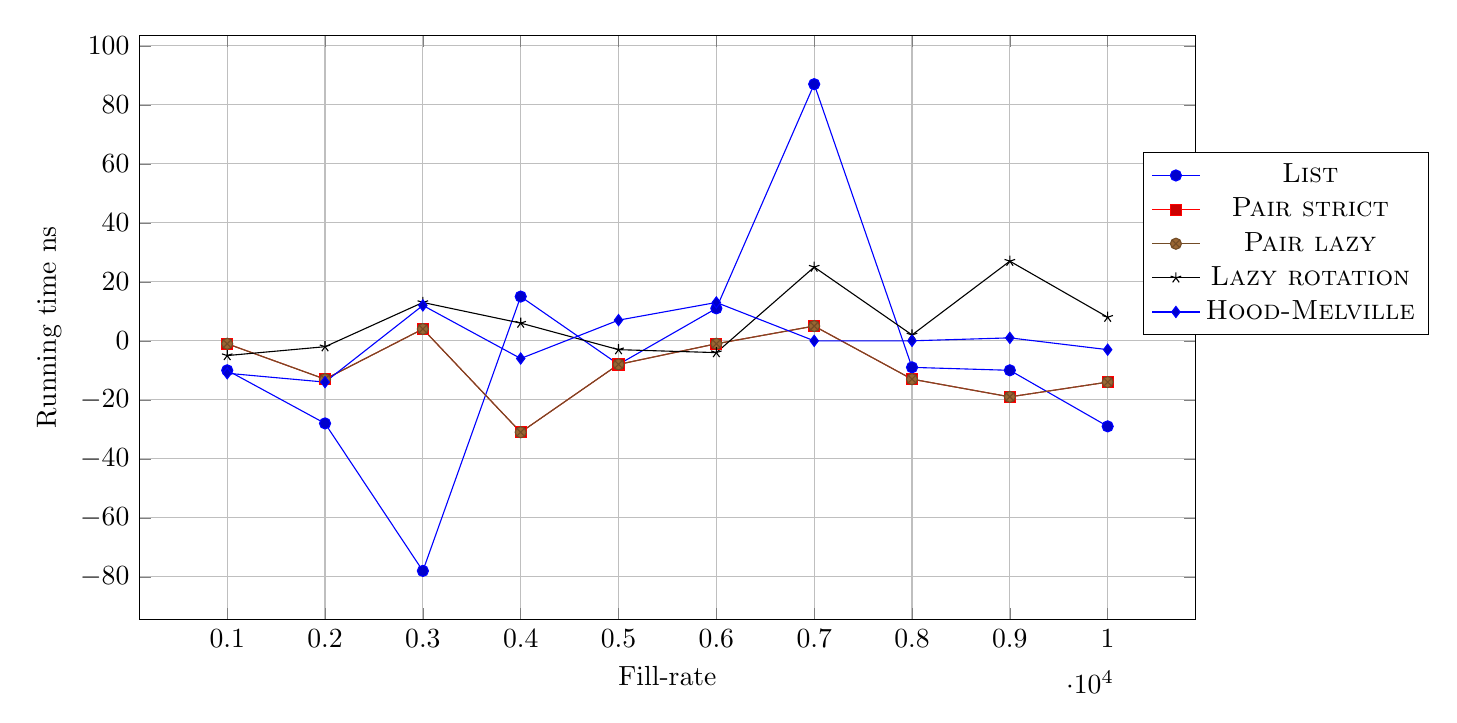
\begin{tikzpicture}
        \begin{axis}[
            xlabel = Fill-rate,
            ylabel = Running time ns,
            height=9cm,
            width=15cm,
            grid=major,
            legend style={
            at={(0.95,0.8)},
            anchor=north west}]            
            legend pos=center west
    	]
    		
    		
    	\addplot coordinates {
(1000,-10)
(2000,-28)
(3000,-78)
(4000,15)
(5000,-8)
(6000,11)
(7000,87)
(8000,-9)
(9000,-10)
(10000,-29)

    	};
        
    	\addlegendentry{\textsc{List}}

                \addplot coordinates {
(1000,-1)
(2000,-13)
(3000,4)
(4000,-31)
(5000,-8)
(6000,-1)
(7000,5)
(8000,-13)
(9000,-19)
(10000,-14)

    	};
        
    	\addlegendentry{\textsc{Pair strict}}

        \addplot coordinates {
(1000,-1)
(2000,-13)
(3000,4)
(4000,-31)
(5000,-8)
(6000,-1)
(7000,5)
(8000,-13)
(9000,-19)
(10000,-14)

    	};
        
    	\addlegendentry{\textsc{Pair lazy}}

        \addplot coordinates {
(1000,-5)
(2000,-2)
(3000,13)
(4000,6)
(5000,-3)
(6000,-4)
(7000,25)
(8000,2)
(9000,27)
(10000,8)

    	};
        
    	\addlegendentry{\textsc{Lazy rotation}}

        \addplot coordinates {
(1000,-11)
(2000,-14)
(3000,12)
(4000,-6)
(5000,7)
(6000,13)
(7000,0)
(8000,0)
(9000,1)
(10000,-3)

    	};
        
    	\addlegendentry{\textsc{Hood-Melville}}

        \end{axis}

    \end{tikzpicture}
    \captionof{figure}{TITEL}
    \label{fig:sample_figure}
\end{minipage}